\section{Sinusformade signaler}
\textbf{HAREC a.\ref{HAREC.a.1.6}\label{myHAREC.a.1.6}}

\begin{figure*}
\begin{center}
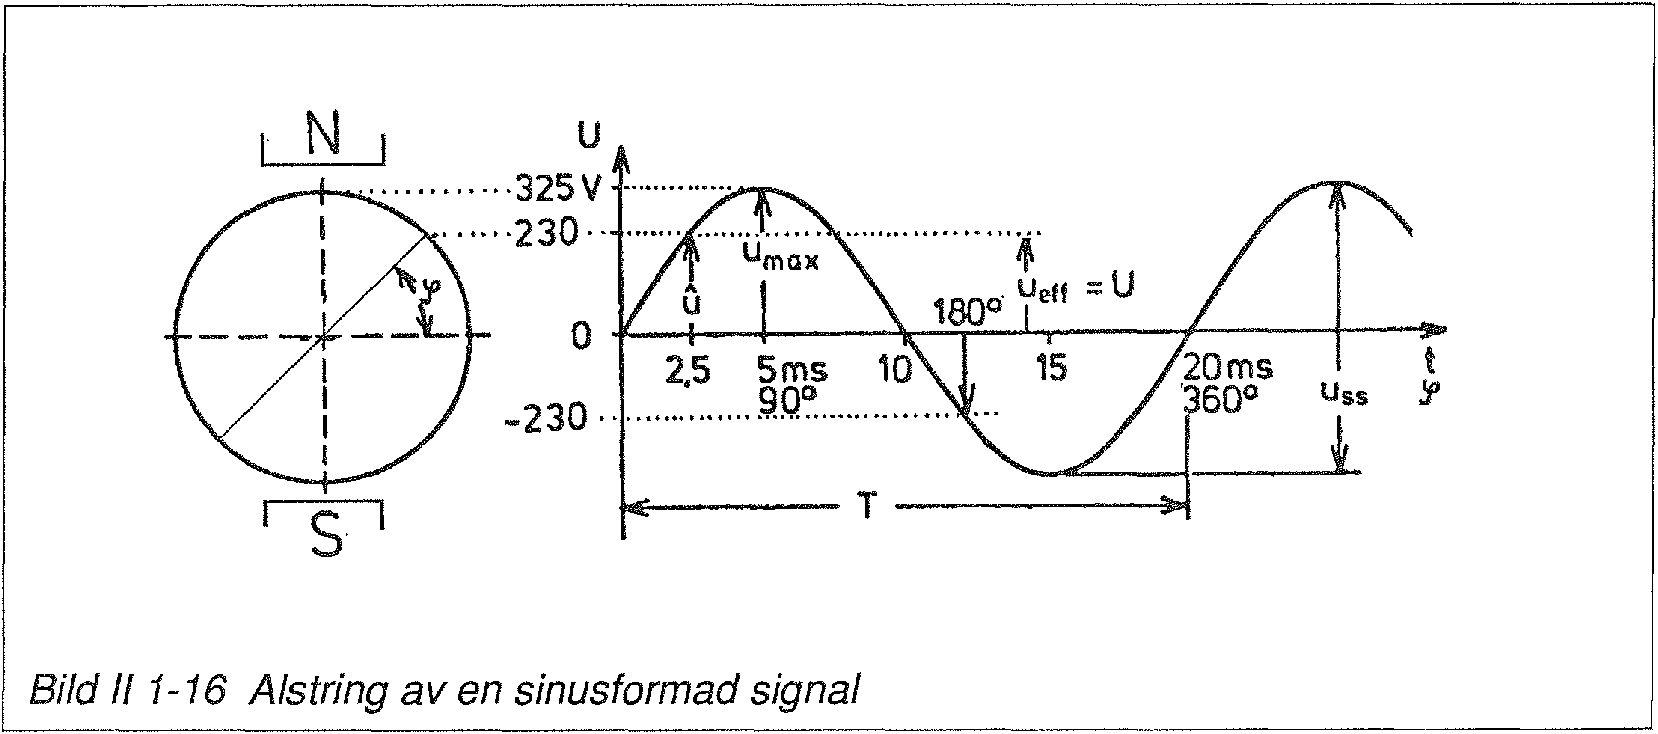
\includegraphics[width=14cm]{images/bild_2_1-16}
\caption{Alstring av en sinusformad signal}
\label{fig:BildII1-16}
\end{center}
\end{figure*}

Bild \ref{fig:BildII1-16}.

\emph{I detta avsnitt behandlas några grundbegrepp inom växelströmsläran. Förloppen
  framställs med vektor- och linjediagram.}

\emph{För närmare beskrivning används sådana begrepp som momentanvärde, toppvärde, topp- till
  toppvärde, effektiwärde, fasläge, fasförskjutning och båghastighet.}

\subsection{Momentanvärde}

Momentanvärdet är storheten på en spänning \(u\), en ström i etc. vid en viss tidpunkt \(t\).
(Storheter som ändrar sig som en funktion av tiden kännetecknas ofta med gemena bokstäver.)

Bilden visar en sinusformad växelspänning med frekvensen \(50 Hz\). Spänningen \(u\) är \(+230 V\) vid tidpunkten 2.5 millisekunder efter en positiv nollgenomgång. Efter totalt \(5 ms\)
uppnås toppvärdet \(u\) d.v.s. \(+325 V\). Efter totalt \(1O ms\) sker en neagativ
nollgenomgång. Efter totalt \(12.5 ms\) är spänningen \(-u\), d.v.s. \(-230 V\) o.s.v.

\subsection{Toppvärde eller amplitud}

Toppvärdet u är det högsta värdet över eller under noll. På bilden är de högsta
värdena \(+325 V\) och \(-325 V\).

\subsection{Topp-till-toppvärde}

Topp-till-toppvärdetuss är summan av toppvärdena över och under noll. På bilden är
detta värde 650 V.

\subsection{Effektivvärde}

Effektivvärdet av en växelspänning \(u\) är det värde, som medför samma effektutveckling
som en likspänning \(U\).

För ett sinusformat förlopp gäller följande samband mellan toppvärdet och effektivvärdet
(det s.k. kvadratiska medelvärdet), vilket motsvarar amplituden vid vinklarna 45,
135, 225 och 270\(\circ\).

\(U=\frac{\hat{u}}{\sqrt{2}}\) \(I=\frac{\hat{i}}{\sqrt{2}}\) (\(\sqrt{2} = 1.414\))

\subsection{Fasläge}

Fasläget är när inom en period, som ett givet momentanvärde uppträder. Tidpunkten för
varje momentanvärde motsvarar en andel av 360\(\circ\) elektriska grader. T.ex. uppnås
värdet volt vid 0\(\circ\), 180\(\circ\) och 360\(\circ\) (= 0\(\circ\)).

\subsection{Bågmått}

I beräkningar av växelströmskretsar används ofta inte vinkelmått för fasläget (gradtal)
utan i stället begreppet bågmått.

I en s.k. enhetskrets med radien \(r = 1\) motsvaras vinkeln 360\(\circ\) av en båge med
längden \(2 \cdot \pi \cdot r= 2 \cdot \pi \cdot 1 = 2 \pi =\) omkretsen
Vid \(f\) perioder per sekund blir båglängden \(= 2\pi f\). Denna storhet kallas båghastigheten
och betecknas med ro (uttalas omega).
\(\omega= 2\pi f\) \([1/s]\)

\subsection{Period}

En period har passerat, när en storhet (spänning, ström o.s.v.) återtagit samma tillstånd
eller värde efter att ha gjort en fullständig växling, t.ex. en hel pendelrörelse eller ett
helt varv vid rotation.

\subsection{Periodtid T}

Periotid T är den tid som åtgår för att strömmen ellerspänningen skall genomlöpa
en period. Periodtiden är det inverterade värdet av frekvensen.

Måttenheten för periodtid är sekund [sj

Periodtid

\((T) = \frac{1}{f}\)

T [s] f[Hz] eller
T [ms] f [kHz] eller
T [ms] f [MHz]

Exempel:

\begin{center}
\begin{tabular}{lll}
\(T_1=\frac{1}{10}\) s & = 0.100 s & = 100 ms (f = 10 Hz)\\
\(T_2=\frac{1}{50}\) s & = 0.020 s & = 20 ms (f = 50 Hz)\\
\(T_3=\frac{1}{1000}\) s & = 0.001 s & = 1 ms (f = 1 kHz)\\
\(T_4=\frac{1}{1000000}\) s & = 0.000001 s & = 1 \(\mu\)s (f = 1 MHz)\\
\end{tabular}
\end{center}

\subsection{Frekvens}

Frekvens är antalet perioder per tidsenhet.

Följande begrepp demonstreras med hjälp av pendeln:

Period = en fullständig fram- och tillbakasvängning i ett system, t.ex. pendelns väg
mellan punkterna 2- 3- 2- 1 - 2- 3- o.s.v.

Periodtid T = tidsåtgången för en fullständig svängning.

Amplitud A = den största avvikelsen från viloläget.

Frekvens f = antal svängningar/tidsenhet.

Sambandet mellan frekvensen f och periodtiden T är

\(f=\frac{1}{T}\) t. ex.

\(5 [H z] = \frac{1}{5} [sekunder]\)

\subsection{Enheten Hertz}

Måttenheten för frekvens är Hertz [Hz].
l formler betecknas frekvensen med f.

\begin{center}
\begin{tabular}{ll}
1 Hz      & = 1 period per sekund (p/s) \\
10 Hz     & = 10 perioder per sekund \\
50 Hz     & = 50 perioder per sekund \\
1 000 Hz  & = \(10^3\) Hz = 1 kHz (kilohertz) \\
1 000 kHz & = \(10^6\) Hz = 1 MHz (megahertz) \\
1 000 MHz & = \(10^9\) Hz = 1 GHz (gigahertz) \\
\end{tabular}
\end{center}

Nätfrekvensen för elkraft är i Europa 50 Hz.

Andra nätfrekvenser förekommer, t.ex. 60Hz i USA.

Frekvensområdet vid överföring av kvalitativt tal och musik, lågfrekvens LF, är mellan ca 16Hz och 16kHz.

Frekvensområdet för talöverföring, t.ex. över telefonlinjer eller kommunikationsradio,
är c:a 300 till 3000 Hz.

Frekvensområdet för radioöverföring, högfrekvens HF, är i huvudsak mellan 50 kHz, s.k.
långvåg, och 100-tals GHz, s.k. mikrovåg.

\subsection{Fasförskjutning}

\begin{figure*}
\begin{center}
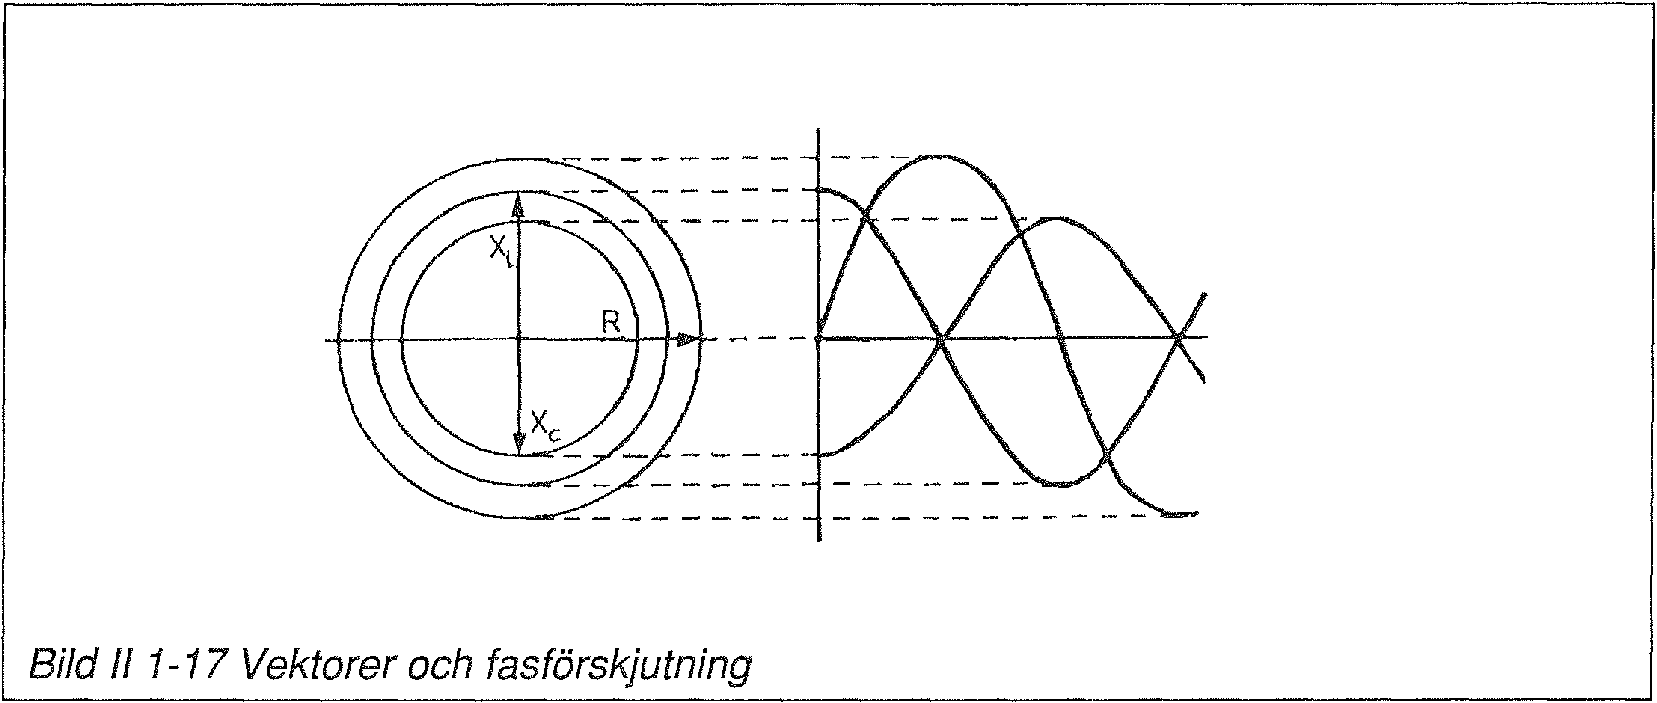
\includegraphics[width=14cm]{images/bild_2_1-17}
\caption{Vektorer och fasförskjutning}
\label{fig:BildII1-17}
\end{center}
\end{figure*}

Bild \ref{fig:BildII1-17}.

Med fasförskjutning menas tidsskillnaden mellan förlopp, t.ex. spänningar och/eller
strömmar. Fasförskjutningen mellan vektorerna kallas även fasvinkel och uttrycks
som ett gradtal mellan 0 och 360°.

\subsection{Vektorer}

En spänning, ström, kraft o.s.v. kan beskrivas som en vektor med en storhet och riktning.
På bilden har vektorerna \(X_L\), \(R\) och \(X_C\) en inbördes fasförskjutning av 90\(\circ\).
De motsvarar spänningsfallen i en krets med en induktor, en resister och en kondensator
kopplade i serie.

Antag att vektorerna roterar i ett oförändrat inbördes läge och med en vinkelhastighet
av \(\omega= 2\pi f\). Systemet roterar då \(360\circ = 2\pi radianer = 1 varv/period\).

Vid varje tidpunkt har vektorsystemet uppnått en viss vridningsvinkeL Momentanvärdet på
vektorernas spänningar avsätts till höger i bilden. Avståndet mellan en vektorspets och
noll-linjen är vektorns momentana värde, som kan vara positivt eller negativt.
